\documentclass[11pt,a4paper]{article}

% ══════════════════════════════════════════════════════════════
% PACKAGES
% ══════════════════════════════════════════════════════════════
\usepackage[margin=2.2cm,top=2.5cm,bottom=2.5cm]{geometry}
\usepackage{amsmath,amssymb}
\usepackage{graphicx}
\usepackage[dvipsnames,svgnames,x11names]{xcolor}
\usepackage{tikz}
\usetikzlibrary{shapes,arrows.meta,positioning,calc,decorations.pathreplacing,shadows,fit}
\usepackage{booktabs}
\usepackage{tabularx}
\usepackage{fancyhdr}
\usepackage{hyperref}
\usepackage{enumitem}
\usepackage{multicol}
\usepackage{tcolorbox}
\tcbuselibrary{skins,breakable}
\usepackage[T1]{fontenc}
\usepackage{titlesec}
\usepackage{float}
\usepackage{setspace}
\usepackage{parskip}
\usepackage{siunitx}

% ══════════════════════════════════════════════════════════════
% COLORS
% ══════════════════════════════════════════════════════════════
\definecolor{qnkpurple}{HTML}{7C3AED}
\definecolor{qnkblue}{HTML}{3B82F6}
\definecolor{qnkcyan}{HTML}{06B6D4}
\definecolor{qnkgreen}{HTML}{10B981}
\definecolor{qnkamber}{HTML}{F59E0B}
\definecolor{qnkred}{HTML}{EF4444}
\definecolor{qnkdark}{HTML}{0F172A}
\definecolor{qnkslate}{HTML}{334155}
\definecolor{qnkgold}{HTML}{D4AF37}
\definecolor{sectioncolor}{HTML}{5B21B6}
\definecolor{boxbg}{HTML}{F5F3FF}
\definecolor{keyboxbg}{HTML}{EFF6FF}
\definecolor{dbred}{HTML}{C0392B}
\definecolor{dborange}{HTML}{E67E22}

% ══════════════════════════════════════════════════════════════
% STYLING
% ══════════════════════════════════════════════════════════════
\hypersetup{
    colorlinks=true,
    linkcolor=qnkpurple,
    urlcolor=qnkblue,
    citecolor=qnkpurple,
    pdfauthor={Q-NarwhalKnight Foundation},
    pdftitle={Dragon Ball Miner x Quillon -- Hardware Cooperation Proposal},
}

\pagestyle{fancy}
\fancyhf{}
\fancyhead[L]{\small\textcolor{qnkslate}{Dragon Ball Miner $\times$ Quillon --- Cooperation Proposal}}
\fancyhead[R]{\small\textcolor{qnkslate}{March 2026}}
\fancyfoot[C]{\small\textcolor{qnkslate}{\thepage}}
\renewcommand{\headrulewidth}{0.4pt}

\titleformat{\section}{\Large\bfseries\color{sectioncolor}}{}{0em}{}[\vspace{-0.5em}\textcolor{qnkpurple}{\rule{\textwidth}{1.5pt}}]
\titleformat{\subsection}{\large\bfseries\color{qnkslate}}{}{0em}{}

% Custom boxes
\newtcolorbox{keyinsight}[1][]{
    enhanced, colback=keyboxbg, colframe=qnkblue, boxrule=1pt, arc=4pt,
    left=10pt, right=10pt, top=8pt, bottom=8pt,
    fonttitle=\bfseries\color{qnkblue}, title={#1},
    shadow={1mm}{-1mm}{0mm}{black!15}
}
\newtcolorbox{highlight}[1][]{
    enhanced, colback=boxbg, colframe=qnkpurple, boxrule=1pt, arc=4pt,
    left=10pt, right=10pt, top=8pt, bottom=8pt,
    fonttitle=\bfseries\color{qnkpurple}, title={#1},
    shadow={1mm}{-1mm}{0mm}{black!15}
}
\newtcolorbox{successbox}[1][]{
    enhanced, colback=green!5, colframe=qnkgreen, boxrule=1pt, arc=4pt,
    left=10pt, right=10pt, top=8pt, bottom=8pt,
    fonttitle=\bfseries\color{qnkgreen!70!black}, title={#1}
}
\newtcolorbox{warningbox}[1][]{
    enhanced, colback=red!5, colframe=qnkred, boxrule=1pt, arc=4pt,
    left=10pt, right=10pt, top=8pt, bottom=8pt,
    fonttitle=\bfseries\color{qnkred}, title={#1}
}

% ══════════════════════════════════════════════════════════════
% DOCUMENT
% ══════════════════════════════════════════════════════════════
\begin{document}

% ──────────────────────────────────────────────────────────────
% TITLE PAGE
% ──────────────────────────────────────────────────────────────
\thispagestyle{empty}
\begin{center}
\vspace*{1.5cm}

% Dual logo area
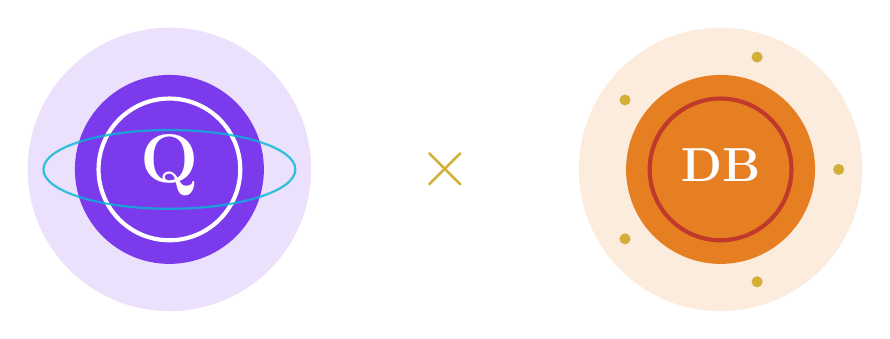
\begin{tikzpicture}
    % Quillon logo
    \fill[qnkpurple!15] (-3.5,0) circle (1.8cm);
    \fill[qnkpurple] (-3.5,0) circle (1.2cm);
    \draw[white, line width=1.5pt] (-3.5,0) circle (0.9cm);
    \node[white, font=\fontsize{28}{28}\selectfont\bfseries] at (-3.5,0.05) {Q};
    \draw[qnkcyan, line width=0.8pt, opacity=0.8] (-3.5,0) ellipse (1.6cm and 0.5cm);

    % Connection symbol
    \node[font=\Huge\bfseries, color=qnkgold] at (0,0) {$\times$};

    % Dragon Ball logo placeholder
    \fill[dborange!15] (3.5,0) circle (1.8cm);
    \fill[dborange] (3.5,0) circle (1.2cm);
    \node[white, font=\fontsize{18}{18}\selectfont\bfseries] at (3.5,0.05) {DB};
    \draw[dbred, line width=1.5pt] (3.5,0) circle (0.9cm);
    % Dragon Ball stars
    \foreach \a in {0,72,...,288} {
        \fill[qnkgold] (3.5,0) ++(\a:1.5cm) circle (2pt);
    }
\end{tikzpicture}

\vspace{1.5cm}

{\fontsize{28}{34}\selectfont\bfseries\textcolor{qnkdark}{Dragon Ball Miner $\times$ Quillon}}

\vspace{0.3cm}

{\Large\textcolor{qnkslate}{Hardware Manufacturing Cooperation Proposal}}

\vspace{0.5cm}

{\large\textcolor{qnkpurple}{\textit{Not Another ASIC --- A New Product Category}}}

\vspace{2cm}

\textcolor{qnkslate}{\rule{8cm}{0.5pt}}

\vspace{0.5cm}

{\large\textbf{Confidential Business Proposal}}

\vspace{0.3cm}

{\textcolor{qnkslate}{March 2026}}

\vspace{2cm}

\begin{tcolorbox}[
    enhanced, colback=qnkpurple!5, colframe=qnkpurple!50,
    boxrule=0.5pt, arc=8pt, width=13cm, center, fontupper=\centering
]
{\small\textcolor{qnkslate}{
\textbf{QUG-V1 Pocket Supercomputer} --- 16-core RISC-V, 17 MH/s @ 9.5W, \$149 retail\\[4pt]
\textbf{QUG-DOCK-16} --- 16-slot enclosure, 272 MH/s @ 200W, each card is a full node\\[4pt]
\textbf{Quillon Forge} --- Dual EPYC 9755, liquid-cooled server, 4$\times$ RTX 5090 option
}}
\end{tcolorbox}

\vfill

{\small\textcolor{qnkslate}{
\textbf{Quillon Foundation} \quad$\cdot$\quad \url{https://quillon.xyz}
}}

\end{center}
\newpage

% ──────────────────────────────────────────────────────────────
% TABLE OF CONTENTS
% ──────────────────────────────────────────────────────────────
\tableofcontents
\newpage

% ══════════════════════════════════════════════════════════════
% SECTION 1: EXECUTIVE SUMMARY
% ══════════════════════════════════════════════════════════════
\section{Executive Summary}

This document proposes a \textbf{hardware manufacturing partnership} between Dragon Ball Miner and the Quillon Foundation. Dragon Ball Miner brings world-class chip fabrication relationships, PCB manufacturing, thermal engineering, and global distribution infrastructure. Quillon brings a production-ready quantum-resistant blockchain with a fully designed custom hardware platform.

\begin{highlight}[The Opportunity in One Sentence]
Dragon Ball Miner has the manufacturing pipeline; Quillon has the hardware design, the blockchain, and the market. Together, we can launch the \textbf{world's first RISC-V mining/node device} with a ready-made network of users.
\end{highlight}

\textbf{Key points:}
\begin{itemize}[leftmargin=1.5em]
    \item Quillon's Proof-of-Work algorithm (BLAKE3 + 100-round VDF) is \textbf{fundamentally incompatible with traditional ASICs}. We are not asking Dragon Ball to build an ASIC.
    \item We \textbf{have} a complete hardware design --- the QUG-V1 Pocket Supercomputer (see companion whitepaper) --- that needs a manufacturing partner.
    \item Each QUG-V1 card is a \textbf{full blockchain node}, not just a hash accelerator. This is an entirely new product category for Dragon Ball.
    \item The \textbf{Quillon Forge} server platform ($\sim$\$24,500--\$42,000) provides an enterprise-tier product line with GPU mining capabilities.
    \item Combined, these products span the entire market: \$149 consumer cards $\to$ \$2,550 DOCK enclosures $\to$ \$42,000 enterprise servers.
\end{itemize}

\begin{keyinsight}[Reference Documents]
This proposal builds on two existing technical whitepapers:
\begin{enumerate}
    \item \textbf{QUG-V1 Pocket Supercomputer} (v1.0.0) --- Full SoC architecture, ISA extensions, thermal analysis, manufacturing BOM, and QUG-DOCK enclosure specifications. \textit{See companion document:} \texttt{qug-v1-pocket-supercomputer.pdf}
    \item \textbf{Q-NarwhalKnight Investor Pitch} (v2, February 2026) --- Complete blockchain overview, tokenomics, competitive landscape, and self-reinforcing success dynamics. \textit{See companion document:} \texttt{investor-pitch-v2.pdf}
\end{enumerate}
Both documents are provided alongside this proposal.
\end{keyinsight}


% ══════════════════════════════════════════════════════════════
% SECTION 2: WHY TRADITIONAL ASICS WON'T WORK
% ══════════════════════════════════════════════════════════════
\section{Why Traditional ASICs Cannot Mine QUG}

Dragon Ball Miner has built highly successful ASICs for Kaspa (kHeavyHash), Alephium (Blake3), NEXA (NexaPow), and Radiant (SHA-512/256). These algorithms share a common property: \textbf{parallelism}. More hashing cores in parallel = more hashes per second = higher probability of finding a valid nonce.

Q-NarwhalKnight's mining algorithm is \textbf{fundamentally different}.

\subsection{The BLAKE3 + 100-Round VDF Chain}

QUG's Proof-of-Work requires evaluating a \textbf{Verifiable Delay Function (VDF)} chain:

\begin{enumerate}[leftmargin=1.5em]
    \item Compute $h_0 = \text{BLAKE3}(\text{challenge} \,\|\, \text{nonce})$
    \item Compute $h_1 = \text{BLAKE3}(h_0)$
    \item Compute $h_2 = \text{BLAKE3}(h_1)$
    \item[] $\vdots$
    \item Compute $h_{99} = \text{BLAKE3}(h_{98})$
    \item If $h_{99} < \text{target}$: valid solution
\end{enumerate}

Each hash \textbf{depends on the previous hash}. This creates a \textbf{sequential chain of 100 BLAKE3 evaluations per nonce candidate}. The chain \textit{cannot} be parallelized --- step $k+1$ requires the output of step $k$.

\begin{warningbox}[The Serialization Barrier]
A GPU with 10{,}000 CUDA cores can evaluate 10{,}000 \textit{different nonces} in parallel --- but each nonce still takes 100 sequential BLAKE3 hashes. A single fast core running at 1.5\,GHz evaluates the same nonce chain in $\sim$0.5\,\textmu s.

\textbf{10{,}000 slow parallel cores $\approx$ 10{,}000 fast sequential cores.}

There is no ``ASIC advantage'' from parallelism because the algorithm is inherently serial \textit{per nonce}. The optimal hardware is many independent fast cores --- which is exactly what the QUG-V1 already is.
\end{warningbox}

\subsection{Why This Matters for Dragon Ball}

Traditional ASIC design focuses on maximizing hash throughput via massive parallelism (hundreds of hashing engines on one die). For QUG:

\begin{center}
\begin{tabular}{@{}p{5cm}p{9cm}@{}}
\toprule
\textbf{Traditional ASIC Approach} & \textbf{Why It Fails for QUG} \\
\midrule
Pack 256 SHA-256 engines on die & Each engine must still do 100 sequential BLAKE3 hashes per nonce --- no throughput gain over 256 independent cores \\
Optimize hash pipeline width & VDF chain is inherently 32-byte wide (BLAKE3 output) --- wider datapaths waste area \\
Remove CPU overhead (no OS) & QUG nodes \textit{must} run a full blockchain node (P2P, storage, consensus) --- a bare-metal hash chip cannot participate in the network \\
\bottomrule
\end{tabular}
\end{center}

\begin{successbox}[The Key Insight]
The QUG-V1 chip design \textit{already is} the optimal hardware for mining QUG. It is a 16-core RISC-V processor with custom \texttt{Xcrypto} BLAKE3 acceleration that achieves 9 cycles per hash. No ASIC redesign would meaningfully improve upon this because \textbf{the bottleneck is sequential latency, not parallel throughput}.

Dragon Ball's value is not in redesigning the chip --- it is in \textbf{manufacturing} the chip we have already designed.
\end{successbox}


% ══════════════════════════════════════════════════════════════
% SECTION 3: THE PRODUCT LINEUP
% ══════════════════════════════════════════════════════════════
\section{The Product Lineup: Three Tiers, One Network}

Quillon has designed a \textbf{complete hardware product line} spanning consumer to enterprise:

\begin{center}
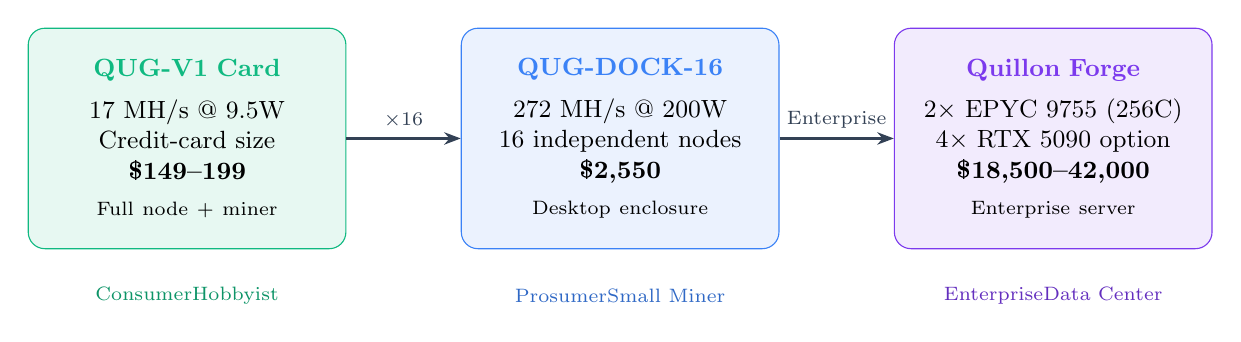
\begin{tikzpicture}[
    tier/.style={draw, rounded corners=6pt, minimum width=4cm, minimum height=2.8cm, font=\small, text width=3.8cm, align=center},
    arrow/.style={-{Stealth[length=6pt]}, thick, qnkslate}
]
    % Tier 1: QUG-V1 Card
    \node[tier, fill=qnkgreen!10, draw=qnkgreen] (card) at (0,0) {
        \textbf{\textcolor{qnkgreen}{QUG-V1 Card}}\\[4pt]
        17 MH/s @ 9.5W\\
        Credit-card size\\
        \textbf{\$149--199}\\[2pt]
        {\scriptsize Full node + miner}
    };

    % Tier 2: QUG-DOCK
    \node[tier, fill=qnkblue!10, draw=qnkblue] (dock) at (5.5,0) {
        \textbf{\textcolor{qnkblue}{QUG-DOCK-16}}\\[4pt]
        272 MH/s @ 200W\\
        16 independent nodes\\
        \textbf{\$2{,}550}\\[2pt]
        {\scriptsize Desktop enclosure}
    };

    % Tier 3: Quillon Forge
    \node[tier, fill=qnkpurple!10, draw=qnkpurple] (forge) at (11,0) {
        \textbf{\textcolor{qnkpurple}{Quillon Forge}}\\[4pt]
        2$\times$ EPYC 9755 (256C)\\
        4$\times$ RTX 5090 option\\
        \textbf{\$18{,}500--42{,}000}\\[2pt]
        {\scriptsize Enterprise server}
    };

    % Arrows
    \draw[arrow] (card) -- node[above, font=\scriptsize] {$\times$16} (dock);
    \draw[arrow] (dock) -- node[above, font=\scriptsize] {Enterprise} (forge);

    % Market labels below
    \node[font=\scriptsize, color=qnkgreen!80!black] at (0,-2) {Consumer\\Hobbyist};
    \node[font=\scriptsize, color=qnkblue!80!black] at (5.5,-2) {Prosumer\\Small Miner};
    \node[font=\scriptsize, color=qnkpurple!80!black] at (11,-2) {Enterprise\\Data Center};
\end{tikzpicture}
\end{center}

\subsection{Tier 1: QUG-V1 Pocket Supercomputer (\$149--199)}

The full technical specification is provided in the companion whitepaper (\texttt{qug-v1-pocket-supercomputer.pdf}). Key specifications:

\begin{center}
\begin{tabular}{@{}ll@{}}
\toprule
\textbf{Parameter} & \textbf{Value} \\
\midrule
Architecture & 16-core heterogeneous RISC-V cluster (RV64GC) \\
Process node & TSMC N5 (5\,nm FinFET) \\
Die size & $\sim$50\,mm$^2$ \\
Mining cores & 8$\times$ RV64 + \texttt{Xcrypto} BLAKE3 acceleration \\
Consensus cores & 4$\times$ RV64 + RVV 1.0 (vector) \\
PQ-Crypto cores & 2$\times$ RV64 + \texttt{Xlattice} (Dilithium5/Kyber1024 NTT) \\
I/O cores & 2$\times$ RV64 + Ethernet MAC + TRNG \\
Mining throughput & 17\,MH/s (8 cores $\times$ 2.12\,MH/s each) \\
Power consumption & 9.5\,W total (mining) \\
Energy efficiency & 1.79\,MH/s/W ($163\times$ better than RTX 4090) \\
Form factor & 85\,mm $\times$ 54\,mm (credit card) \\
Interface & USB-C (power + Ethernet-over-USB) \\
SoC cost (10K vol.) & \$25--35 \\
Retail price & \$149--199 \\
\bottomrule
\end{tabular}
\end{center}

\textbf{Critical differentiator:} Each QUG-V1 card runs a \textbf{complete Q-NarwhalKnight full node} --- its own copy of the blockchain, its own libp2p peer identity, its own vote in DAG-Knight consensus. This is not a USB hash stick. It is a pocket supercomputer that mines \textit{and} validates \textit{and} routes transactions \textit{and} participates in consensus.

\subsection{Tier 2: QUG-DOCK-8 and QUG-DOCK-16 (\$99--199 dock only)}

\begin{center}
\begin{tabular}{@{}lcc@{}}
\toprule
\textbf{Specification} & \textbf{QUG-DOCK-8} & \textbf{QUG-DOCK-16} \\
\midrule
Card slots & 8 & 16 \\
Mining throughput & 136\,MH/s & 272\,MH/s \\
Network nodes & 8 independent & 16 independent \\
Backplane & PCIe Gen3 $\times$4/slot & PCIe Gen3 $\times$4/slot \\
Network switch & Managed GbE (100\,Mbps/slot) & Managed GbE (100\,Mbps/slot) \\
Power (cards + dock) & 91\,W & 167\,W \\
Enclosure & Desktop form factor & Desktop form factor \\
Dock price (no cards) & \$99--129 & \$149--199 \\
Full system price & $\sim$\$1{,}300 & $\sim$\$2{,}550 \\
\bottomrule
\end{tabular}
\end{center}

Throughput scales \textbf{linearly}: $H_{\text{dock}}(N) = N \times 17\,\text{MH/s}$, with zero inter-card coordination overhead. Each card mines on independent nonce ranges.

\subsection{Tier 3: Quillon Forge Enterprise Server (\$18,500--42,000)}

The Quillon Forge is a liquid-cooled dual-socket EPYC server designed for enterprise mining, AI inference, and full-node operation. Full specification in \texttt{QUILLON\_FORGE\_MANUFACTURING\_PIPELINE.md}.

\begin{center}
\begin{tabular}{@{}lp{9cm}@{}}
\toprule
\textbf{Configuration} & \textbf{Specifications \& Price} \\
\midrule
Base (CPU-only) & 2$\times$ AMD EPYC 9755 (256 cores total), 512GB DDR5, 2$\times$3.84TB NVMe, liquid-cooled --- \textbf{\$18,500} \\
GPU Standard & + 2$\times$ NVIDIA RTX 5090 (2$\times$32GB VRAM) --- \textbf{\$24,500} \\
GPU Pro & + 4$\times$ NVIDIA RTX 5090 (4$\times$32GB VRAM) --- \textbf{\$28,500} \\
AI Research & + 2$\times$ NVIDIA A100 80GB --- \textbf{\$32,000} \\
AI Fleet & + 4$\times$ NVIDIA L40 48GB --- \textbf{\$42,000} \\
\bottomrule
\end{tabular}
\end{center}

\textbf{GPU mining integration:} As of March 2026, the Q-NarwhalKnight standalone miner and Slint desktop wallet both support OpenCL GPU mining with the same BLAKE3+VDF kernel. GPU-equipped Forge servers can mine with both CPU threads \textit{and} GPU simultaneously, maximizing hardware utilization.

\begin{keyinsight}[Why Upgrade Forge with More GPUs]
The standalone \texttt{q-miner} and the Slint wallet now both support multi-GPU OpenCL mining. Each RTX 5090 provides significant additional hashrate alongside the 256 CPU cores. The GPU Pro (4$\times$ RTX 5090) configuration is particularly compelling for operators who want maximum hashrate from a single managed server. The \textbf{GPU mining software is production-ready today} --- the hardware just needs to be offered with more GPU options.
\end{keyinsight}

The Forge is tokenized as the \textbf{\$FORGE RWA token} on Q-NarwhalKnight (500 total supply, burn-to-redeem for a physical machine). This creates a secondary market for Forge servers and integrates hardware sales directly into the blockchain ecosystem.


% ══════════════════════════════════════════════════════════════
% SECTION 4: WHERE DRAGON BALL FITS
% ══════════════════════════════════════════════════════════════
\section{Where Dragon Ball Fits: Manufacturing Partner}

\subsection{Dragon Ball's Core Competencies}

Dragon Ball Miner has demonstrated excellence in exactly the capabilities Quillon needs to bring the QUG-V1 to market:

\begin{center}
\begin{tabular}{@{}p{4.5cm}p{9.5cm}@{}}
\toprule
\textbf{Dragon Ball Capability} & \textbf{QUG-V1/DOCK Application} \\
\midrule
Chip fabrication relationships & TSMC/Samsung access for the 5\,nm RISC-V SoC tape-out \\
PCB design \& manufacturing & QUG-V1 credit-card PCB, DOCK backplane, edge connectors \\
Thermal engineering & 9.5W passive cooling for card, 200W active cooling for DOCK-16 \\
Enclosure design & DOCK-8/DOCK-16 desktop enclosures, fan/airflow optimization \\
Power delivery design & USB-C PD for single card, internal PSU for DOCK \\
Quality assurance \& testing & Burn-in testing, MTBF validation, RoHS/CE/FCC compliance \\
Global distribution & Retail and wholesale channels to mining community worldwide \\
Volume pricing leverage & SoC cost reduction below \$25 at Dragon Ball's order volumes \\
\bottomrule
\end{tabular}
\end{center}

\subsection{What Quillon Provides}

\begin{center}
\begin{tabular}{@{}p{4.5cm}p{9.5cm}@{}}
\toprule
\textbf{Quillon Contribution} & \textbf{Details} \\
\midrule
Complete SoC design & RTL-ready 16-core RISC-V design with Xcrypto + Xlattice extensions \\
Firmware \& OS & Bare-metal mining firmware + Linux full-node stack \\
Blockchain network & 500{,}000+ LOC production blockchain with live network \\
Mining software & Production GPU + CPU miners (OpenCL, multi-device) \\
Wallet software & Desktop (Slint) + Web wallet with built-in miner \\
User base & Active mining community on quillon.xyz \\
Tokenized distribution & \$FORGE RWA tokens for Forge servers; similar model available for QUG-V1 \\
\bottomrule
\end{tabular}
\end{center}


% ══════════════════════════════════════════════════════════════
% SECTION 5: A NEW PRODUCT CATEGORY
% ══════════════════════════════════════════════════════════════
\section{Not Another ASIC --- A New Product Category}

\begin{highlight}[Why This Is Different From Everything Dragon Ball Has Built]
Every product Dragon Ball has shipped --- the KAS miner, the ALPH miner, the NEXA miner --- is a \textbf{dedicated hashing device}. It does one thing: compute hashes. It has no storage, no networking intelligence, no blockchain state.

The QUG-V1 is a \textbf{complete computer}. It runs a full operating system, stores its own copy of the blockchain, has its own cryptographic identity, participates in peer-to-peer networking, validates transactions, votes in consensus, \textit{and} mines. Selling QUG-V1 cards is like selling miniature blockchain servers, not hash sticks.
\end{highlight}

\subsection{The Market Positioning}

\begin{center}
\begin{tabular}{@{}p{3.5cm}cccc@{}}
\toprule
 & \textbf{Traditional ASIC} & \textbf{GPU Miner} & \textbf{QUG-V1} & \textbf{Raspberry Pi} \\
\midrule
Mines & Yes & Yes & Yes & Barely \\
Full node & No & Optional & \textcolor{qnkgreen}{\textbf{Always}} & Yes \\
Consensus vote & No & No & \textcolor{qnkgreen}{\textbf{Yes}} & Yes \\
Peer identity & No & No & \textcolor{qnkgreen}{\textbf{Yes}} & Yes \\
Form factor & Rack/shelf & Desktop & \textcolor{qnkgreen}{\textbf{Credit card}} & SBC \\
Power & 500--3000W & 300--1000W & \textcolor{qnkgreen}{\textbf{9.5W}} & 5--15W \\
QUG hashrate & N/A & $\sim$5\,MH/s & \textcolor{qnkgreen}{\textbf{17\,MH/s}} & $\sim$200\,kH/s \\
Price & \$3{,}000--15{,}000 & \$1{,}500--5{,}000 & \textcolor{qnkgreen}{\textbf{\$149--199}} & \$80 \\
\bottomrule
\end{tabular}
\end{center}

\textbf{Each QUG-V1 sold strengthens the network.} Unlike traditional ASICs that centralize hashrate without contributing nodes, every QUG-V1 card adds a full peer to the decentralized network. This makes the product \textit{aligned} with the blockchain's philosophy rather than adversarial to it.

\subsection{Dragon Ball's New Customer Segment}

Dragon Ball's current customers are industrial miners who buy rack-mounted ASIC units. The QUG-V1 opens a \textbf{new market segment}:

\begin{itemize}[leftmargin=1.5em]
    \item \textbf{Individual hobbyists} who want a plug-and-play miner for \$149
    \item \textbf{Crypto enthusiasts} who want to run a full node without managing a server
    \item \textbf{Small businesses} who want a DOCK-16 for quiet office mining
    \item \textbf{Existing Dragon Ball customers} who want to diversify into QUG mining alongside KAS/ALPH
    \item \textbf{Institutional operators} who want Quillon Forge servers with GPU mining
\end{itemize}

This is \textbf{additive} to Dragon Ball's existing business, not cannibalistic.


% ══════════════════════════════════════════════════════════════
% SECTION 6: ECONOMICS
% ══════════════════════════════════════════════════════════════
\section{Economics and Revenue Model}

\subsection{QUG-V1 Card Economics}

\begin{center}
\begin{tabular}{@{}lrr@{}}
\toprule
\textbf{Component} & \textbf{Cost (10K vol.)} & \textbf{Share} \\
\midrule
QUG-V1 SoC (TSMC N5, 50\,mm$^2$) & \$25--35 & 45\% \\
LPDDR5 2GB & \$8--12 & 14\% \\
eMMC 32GB + NOR 16MB & \$6--9 & 10\% \\
PCB (6-layer HDI, 85$\times$54mm) & \$4--6 & 7\% \\
USB-C PD controller + connectors & \$3--5 & 6\% \\
Passive cooling (heatspreader) & \$2--3 & 4\% \\
Assembly \& test & \$5--8 & 10\% \\
Packaging \& shipping & \$2--3 & 4\% \\
\midrule
\textbf{Total BOM + Manufacturing} & \textbf{\$55--81} & 100\% \\
\midrule
Retail price (2$\times$ markup) & \$149--199 & --- \\
\textbf{Gross margin} & \textbf{52--59\%} & --- \\
\bottomrule
\end{tabular}
\end{center}

\subsection{QUG-DOCK Economics}

\begin{center}
\begin{tabular}{@{}lrr@{}}
\toprule
\textbf{Component} & \textbf{DOCK-8} & \textbf{DOCK-16} \\
\midrule
Managed Ethernet switch IC & \$15 & \$15 \\
Backplane PCB + edge connectors & \$12 & \$20 \\
Enclosure (aluminum, injection-molded) & \$15 & \$25 \\
PSU (120W / 250W) & \$10 & \$18 \\
Fans + thermal management & \$5 & \$8 \\
Controller MCU + firmware & \$4 & \$4 \\
Assembly \& test & \$8 & \$12 \\
\midrule
\textbf{Total BOM} & \textbf{\$69} & \textbf{\$102} \\
Retail price & \$99--129 & \$149--199 \\
Gross margin & 30--47\% & 32--49\% \\
\midrule
\textbf{Full system (cards + dock)} & & \\
Cards (8$\times$ or 16$\times$ @ \$149) & \$1{,}192 & \$2{,}384 \\
+ Dock & \$99--129 & \$149--199 \\
\textbf{Full system retail} & \textbf{$\sim$\$1{,}300} & \textbf{$\sim$\$2{,}550} \\
\bottomrule
\end{tabular}
\end{center}

\subsection{Revenue Projections (Conservative)}

\begin{center}
\begin{tabular}{@{}lcccr@{}}
\toprule
\textbf{Product} & \textbf{Year 1 Units} & \textbf{ASP} & \textbf{Revenue} & \textbf{Gross Profit} \\
\midrule
QUG-V1 Card & 10{,}000 & \$175 & \$1{,}750{,}000 & \$962{,}500 \\
QUG-DOCK-8 & 500 & \$115 & \$57{,}500 & \$23{,}000 \\
QUG-DOCK-16 & 300 & \$175 & \$52{,}500 & \$22{,}050 \\
Quillon Forge & 50 & \$26{,}000 & \$1{,}300{,}000 & \$598{,}000 \\
\midrule
\textbf{Total Year 1} & & & \textbf{\$3{,}160{,}000} & \textbf{\$1{,}605{,}550} \\
\bottomrule
\end{tabular}
\end{center}


% ══════════════════════════════════════════════════════════════
% SECTION 7: PROPOSED COOPERATION STRUCTURE
% ══════════════════════════════════════════════════════════════
\section{Proposed Cooperation Structure}

\subsection{Option A: Manufacturing Partnership}

Dragon Ball manufactures the QUG-V1, DOCK, and Forge hardware under license from Quillon:

\begin{itemize}[leftmargin=1.5em]
    \item \textbf{Dragon Ball role}: Tape-out management, PCB manufacturing, assembly, QA, distribution
    \item \textbf{Quillon role}: SoC RTL design, firmware, blockchain software, brand, community
    \item \textbf{Revenue split}: Negotiable (e.g., 60/40 or 70/30 in favor of manufacturer)
    \item \textbf{Branding}: Co-branded ``Dragon Ball $\times$ Quillon'' or Quillon brand with ``Manufactured by Dragon Ball''
\end{itemize}

\subsection{Option B: Joint Venture}

Form a joint entity (``Quillon Hardware'' or similar) that owns the hardware product line:

\begin{itemize}[leftmargin=1.5em]
    \item Shared investment in tape-out costs ($\sim$\$2--5M for TSMC N5 NRE)
    \item Shared ownership of manufactured inventory
    \item Dragon Ball contributes manufacturing infrastructure; Quillon contributes IP and software
    \item Profits shared per equity stake
\end{itemize}

\subsection{Option C: OEM/ODM Arrangement}

Dragon Ball produces QUG-V1 hardware as an OEM, selling units to Quillon at cost + margin:

\begin{itemize}[leftmargin=1.5em]
    \item Simplest legal structure
    \item Dragon Ball earns manufacturing margin; Quillon earns retail margin
    \item Quillon handles all branding, sales, and distribution
    \item Dragon Ball can also sell through their own channels under co-brand
\end{itemize}


% ══════════════════════════════════════════════════════════════
% SECTION 8: TIMELINE
% ══════════════════════════════════════════════════════════════
\section{Development and Manufacturing Timeline}

\begin{center}
\begin{tabular}{@{}p{2.5cm}p{11.5cm}@{}}
\toprule
\textbf{Phase} & \textbf{Milestone} \\
\midrule
\textbf{2026 Q2} & Partnership agreement signed. Joint review of QUG-V1 RTL design. Dragon Ball provides DFM (Design for Manufacturability) feedback. \\
\textbf{2026 Q3} & FPGA prototype validation. Xcrypto BLAKE3 extension verified at 100\,MHz ($\sim$1\,MH/s). Firmware boots and mines on FPGA. \\
\textbf{2026 Q4} & PCB design finalized (credit-card form factor). DOCK-8/DOCK-16 enclosure prototyping. \\
\textbf{2027 Q1} & TSMC 7\,nm tape-out (conservative first silicon). Target: 10\,MH/s at 12\,W. \\
\textbf{2027 Q2} & First silicon bring-up. Firmware porting from FPGA to silicon. Thermal validation. \\
\textbf{2027 Q3} & TSMC 5\,nm tape-out (production die). Volume manufacturing begins. First \$149 retail units ship. QUG-DOCK-8 and DOCK-16 ship alongside. \\
\textbf{2027 Q4} & Scale to 10{,}000+ units/quarter. Global retail distribution. \\
\bottomrule
\end{tabular}
\end{center}

\textbf{Note:} The FPGA prototype phase (2026 Q3) can proceed immediately --- it requires only FPGA development boards, not TSMC access. This allows validating the design and mining software before committing to a tape-out.


% ══════════════════════════════════════════════════════════════
% SECTION 9: THE NETWORK EFFECT
% ══════════════════════════════════════════════════════════════
\section{The Network Effect: Why Hardware Sales Compound}

Unlike traditional ASIC sales (where the manufacturer's relationship with the customer ends at delivery), QUG-V1 sales create a \textbf{compounding network effect}:

\begin{center}
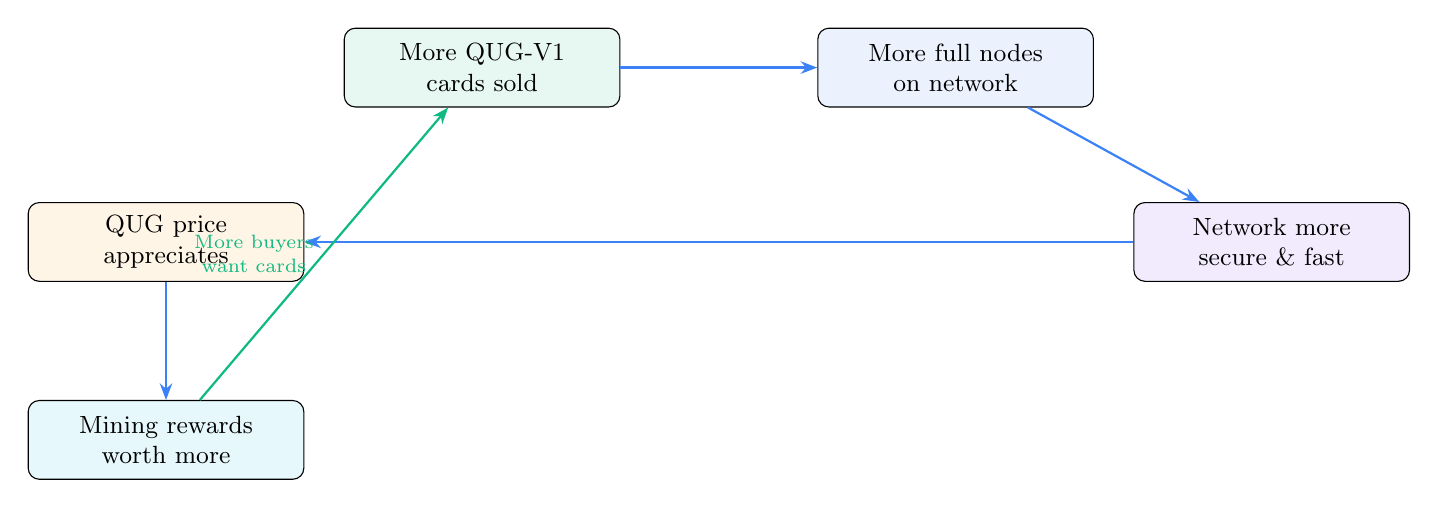
\begin{tikzpicture}[
    node distance=2cm,
    every node/.style={align=center, font=\small},
    arrow/.style={-{Stealth[length=6pt]}, thick, qnkblue}
]
    \node[draw, rounded corners, fill=qnkgreen!10, minimum width=3.5cm, minimum height=1cm] (sell) {More QUG-V1\\cards sold};
    \node[draw, rounded corners, fill=qnkblue!10, minimum width=3.5cm, minimum height=1cm, right=2.5cm of sell] (nodes) {More full nodes\\on network};
    \node[draw, rounded corners, fill=qnkpurple!10, minimum width=3.5cm, minimum height=1cm, below right=1.2cm and 0.5cm of nodes] (secure) {Network more\\secure \& fast};
    \node[draw, rounded corners, fill=qnkamber!10, minimum width=3.5cm, minimum height=1cm, below left=1.2cm and 0.5cm of sell] (value) {QUG price\\appreciates};
    \node[draw, rounded corners, fill=qnkcyan!10, minimum width=3.5cm, minimum height=1cm, below=1.5cm of value] (demand) {Mining rewards\\worth more};

    \draw[arrow] (sell) -- (nodes);
    \draw[arrow] (nodes) -- (secure);
    \draw[arrow] (secure) -- (value);
    \draw[arrow] (value) -- (demand);
    \draw[arrow, qnkgreen] (demand) -- node[left] {\scriptsize More buyers\\[-2pt]\scriptsize want cards} (sell);
\end{tikzpicture}
\end{center}

\textbf{Every card sold increases the value of every other card.} This is the opposite of traditional ASIC economics, where more hashrate on the network \textit{decreases} individual mining profitability. With QUG-V1, more cards = more nodes = stronger network = higher QUG value = more profitable mining for everyone.


% ══════════════════════════════════════════════════════════════
% SECTION 10: CONCLUSION
% ══════════════════════════════════════════════════════════════
\section{Conclusion}

\begin{center}
\begin{tcolorbox}[
    enhanced, colback=qnkpurple!8, colframe=qnkpurple,
    boxrule=1.5pt, arc=8pt, width=14cm,
    shadow={2mm}{-2mm}{0mm}{black!20}
]
\begin{center}
{\Large\bfseries\textcolor{qnkpurple}{Dragon Ball has the factory.\\Quillon has the blueprint and the network.}}

\vspace{0.5cm}

{\large\textcolor{qnkslate}{Together, we launch the world's first RISC-V\\blockchain supercomputer in credit-card form factor.}}

\vspace{0.5cm}

{\small\textcolor{qnkslate}{\textit{Not an ASIC. Not a GPU. Something entirely new.}}}
\end{center}
\end{tcolorbox}
\end{center}

\vspace{1cm}

\textbf{Next steps:}
\begin{enumerate}[leftmargin=1.5em]
    \item Review this proposal and the companion whitepapers
    \item Schedule a technical deep-dive call to review the QUG-V1 RTL design
    \item Sign mutual NDA for detailed IP sharing
    \item Agree on cooperation structure (Option A, B, or C)
    \item Begin FPGA prototype phase (can start immediately)
\end{enumerate}

\vfill

\begin{center}
\textcolor{qnkslate}{\rule{8cm}{0.5pt}}

\vspace{0.3cm}

{\small
\textbf{Website:} \url{https://quillon.xyz} \quad$\cdot$\quad \textbf{Live Network:} \url{https://quillon.xyz}

\vspace{0.2cm}

\textbf{Companion Documents:}\\
\texttt{qug-v1-pocket-supercomputer.pdf} --- QUG-V1 Full Technical Whitepaper\\
\texttt{investor-pitch-v2.pdf} --- Q-NarwhalKnight Investor Pitch \& Technical Overview
}
\end{center}

\vspace{0.5cm}

\begin{center}
\begin{minipage}{13cm}
{\scriptsize\textcolor{gray}{
\textbf{Confidentiality Notice:} This document contains proprietary information of the Quillon Foundation. It is provided solely for the purpose of evaluating a potential business relationship with Dragon Ball Miner. Unauthorized distribution, reproduction, or disclosure is strictly prohibited. The financial projections contained herein are estimates based on current market conditions and manufacturing cost assumptions; actual results may vary materially. Hardware specifications are based on current design targets and may change during the engineering and manufacturing process.
}}
\end{minipage}
\end{center}

\end{document}
